\documentclass[11pt]{article}
\usepackage{graphicx}
\usepackage{float}
\usepackage{cite}
\usepackage{url}
\usepackage[title]{appendix}
\usepackage{listings}
\graphicspath{ {images/} }
\begin{document}

\title{An Empirical Analysis of the Backtracking Algorithm in Solving a 9 × 9 Sudoku Puzzle}
\author{Tristan Le Forestier – 1835635 \and Michael Gomes – 1644868 \and Tristen Paul – 1826461}
\maketitle

\newpage

\section{Aims}
\begin{enumerate}
\item To measure the performance of the backtracking algorithm in solving a Sudoku puzzle and compare the results to theoretical analysis
\item To determine the improvement in performance of the backtracking algorithm achieved by using a stack-based implementation as compared to the recursive approach. 
\item To determine the improvement in performance by running each algorithm on computer systems with different specifications and hardware.
\item To investigate how the number of unpopulated cells in a sudoku puzzle contributes to the runtime of the backtracking algorithm.
\end{enumerate}

\section{Summary of Theory}
\subsection{Research Paper 1}Sudoku is a number based combinatoric puzzle, which relies on the use of logic to solve. 
It usually comprises of a 9×9 square grid which is then subdivided into 9 3×3 blocks. 
Within these blocks there are particular cells which have filled in numbers from the set {1,2,3,4,5,6,7,8,9} which are given as clues. 
The aim of the puzzle is to fill in empty cells such that each row, column and block contain each number in the set only once.
 \cite{DJVP}Other variations of the puzzle exist, however are not pertinent to the scope of this report.  
The backtracking method of solving a Sudoku puzzle attempts to find a solution by sequentially trying different numbers until a solution is found.
 If the algorithm is unable to find a valid solution with the current number combination it “backtracks” and attempts to find a solution using another number. 
 This is a simple brute force method and is the same algorithm which is analysed in this paper. \cite{DJVP}  

\subsection{Research Paper 2}
In paper \cite{SJAR}, it is stated that in order to guarantee that a unique solution to a sudoku puzzle can be computed using the backtracking algorithm,
 a minimum of 17 numbers have to be given as clues. This means that any sudoku puzzle which contains less than 17 clues has to contain at least two unique solutions. 
This paper further outlines another backtracking method to solve a sudoku puzzle which makes use of backtracking combined with column permutations which vastly improved the efficiency and
 runtime of this sudoku solver when compared to the original backtracking algorithm.

\subsection{Research Paper 3}
Aljohani and Smith \cite{AAWS} assert that a sudoku puzzle is an NP-Complete problem. 
 NP stands for nondeterministic polynomial and means that the optimal solution of a generalized sudoku puzzle cannot be determined in polynomial time. 
 The time complexity of a 9-by-9 puzzle is exponential and is given by O($9^N$) where N is the number of empty cells in the puzzle and is stated as being NP-hard. 
A parallel implementation of the backtracking algorithm was implemented by the authors of this paper.
 They discovered that the strong scaling speed up and efficiency of the algorithm is low and inconsistent when running on more than two cores. 
 This indicates that a serial implementation of the backtracking algorithm will be the most appropriate choice for an empirical analysis. 


\subsection{Research Paper 4}
There are several implementations of the simple backtracking algorithm stated in paper \cite{LCGL}.
 The standard simple backtracking algorithm uses the standard method previously outlined. The backtracking algorithm with heuristic moves adds additional 
 complexity to the backtracking algorithm by basing its choice of number on extra conditions such as the number of occurrences of a number already in the puzzle as well as the
  conditions which form the core rules of sudoku. 
It was found that the additional conditions in the heuristic implementation improved the run time of the algorithm in certain cases, 
however due to the NP-complete nature of the sudoku problem this improvement was not uniform across all attempts and puzzle variations. 


\section{Experimental Methodology}
\subsection{Choice of Metric for Analysis}
For this empirical analysis the most appropriate unit to measure performance is time. 
Utilising the website \cite{GGRL}, we will generate sudoku puzzles to be solved from categories of difficulty of easy, medium, hard and expert. 
Three puzzles from each category will be tested and the results averaged in order to reduce the effect of experimental error. 
We will run these numerous puzzles on two different backtracking algorithms (our stack implementation vs recursive implementation) and on two different machines of different specifications.
We will test both the stack and recursive backtracking algorithms using different sizes of n where n is the number of missing elements in a particular sudoku 
puzzle to see how the number of missing elements affects runtime. The values of n will be in the range {5, 10, 15, 20, … 60}.
 This range was chosen due to the theoretical analysis in paper \cite{SJAR} which determined that a minimum of 17 clues are needed in order to guarantee a singular unique 
 solution of a 9-by-9 sudoku puzzle. These results will then be compared to the theoretical time complexity of a 9-by-9 sudoku puzzle. We will run these tests on a singular computer system.

\subsection{Implementation}
The sudoku solver algorithm used in this experiment is implemented in Java using Integer and Characters Stacks provided in the Java.util package (Appendix A) and using Recursion (Appendix B).

\vspace{5mm} %5mm vertical space
These implementations are designed to run sequentially with no parallelized elements in order to ensure that the algorithms run on a single core. 
Whilst not the most efficient method of implementation, this serves to improve the accuracy of the results and allows for improved and more comparable time results as the aim 
is to investigate the growth rate of the algorithm.

\vspace{5mm} %5mm vertical space
The result data is generated from a custom implementation of a Timer class (Appendix C) which makes use of the nanoTime() function from the Java.lang.System package in 
order to obtain the most precise runtime of the algorithm. This timer is started after data initialisation and stopped immediately after the algorithm has finished running. 
The data for each iteration is then written to file before another iteration is run.

\vspace{5mm} %5mm vertical space
The experiment used to determine the runtime of the backtracking algorithm with missing cells makes use of the same stacks (Appendix D) and recursive (Appendix E) iterations. 
Both implementations are run using the same completed sudoku puzzle and the choice of which cells to zero makes use of the Random class provided in the Java.util package with a
 constant seed to ensure reliable results.

\section{Hardware}
For this test we will be using two different computer systems for testing:
\begin{enumerate}
\item Ryzen 7 1800X @ 3.60GHz 32GB RAM
\item Intel i3 3227U @ 1.90GHz 4GB RAM
\end{enumerate}
These machines were chosen as they are easily accessible with varying hardware capacities and can be dedicated to generating test data for extended periods of time with minimal 
interference from other tasks and programs. Machines with different clock speeds, system specs and core counts were chosen to demonstrate the runtime and growth rate of the 
backtracking algorithm to prove that the efficiency of the serial implementation is independent of these factors.  

\section{Presentation of Results}
%Tables%
\subsection{Tables}

\begin{figure}[H]
\centering
\begin{tabular}{|l|l|l|l|r|}
\hline
Input & Time 1(ms) & Time 2(ms) & Time 3(ms) & Average(ms)\\
\hline
easy1	& 0,6472  & 0,6357 & 0,6297	& 0,637533333\\
easy2   & 1,0356  & 1,1417 & 1,0696	& 1,0823\\
easy3	& 1,0323  &	1,0189 & 1,0266	& 1,025933333\\
medium1	& 1,2326  &	1,258 &	1,2582	& 1,2496\\
medium2	& 1,3956  &	1,3889 & 1,3528	& 1,3791\\
medium3	& 5,2118  &	5,64 & 5,3695	& 5,4071\\
hard1   & 27,6571 & 30,404 & 27,3336 & 28,4649\\
hard2	& 9,8921  & 10,3453 & 10,2752 & 10,17086667\\
hard3   & 12,0058 & 11,9644 & 12,2545	& 12,0749\\
expert1	& 594,4535 &	617,2143 & 708,5641	& 640,0773\\
expert2	& 91,756 &	112,6508 &	104,1651	& 102,8573\\
expert3	& 124,9082	& 123,0565 &	125,9075  &	124,6240667\\
\hline
Average of Average Times(ms) & & & &77,420908336\\
\hline
\end{tabular}
\caption{Times taken to get the correct output for the specific input on computer system 1 using the algorithm with stacks.}
\end{figure}

\begin{figure}[H]
\centering
\begin{tabular}{|l|l|l|l|r|}
\hline
Input & Time 1(ms) & Time 2(ms) & Time 3(ms) & Average(ms)\\
\hline
easy1	& 4,430882 &	3,784991 & 3,944006 &	4,053293\\
easy2	& 6,96370	&5,652807&	6,924808&	6,513772\\	
easy3	& 6,054909	&6,45403	&6,859152&	6,45603\\
medium1	& 7,165968	&6,961612	&6,829134&	6,985571\\
medium2	&7,461408	&6,176058	&9,128067&	7,588511\\
medium3	&23,8821	&23,324926	&24,423254&	23,87676\\
hard1	&106,615539	&111,785826&	105,675045&	108,02547\\
hard2	&50,003546	&44,773057	&44,10117&	46,292591\\
hard3	&54,056567	&51,047888&	53,86028&	52,988245\\
expert1	&1516,464504	&1644,453756&	1859,542042&	1673,486767\\
expert2	&334,91947	&337,997903&	346,783929&	339,900434\\
expert3	&390,37573	&418,382812&	422,406223&	410,388255\\
\hline
Average of Average Times(ms) & & & &223,879642\\
\hline
\end{tabular}
\caption{Times taken to get the correct output for the specific input on computer system 2 using the algorithm with stacks.}
\end{figure}

\begin{figure}[H]
\centering
\begin{tabular}{|l|l|l|l|r|}
\hline
Input & Time 1(ms) & Time 2(ms) & Time 3(ms) & Average(ms)\\
\hline
easy1	 & 0,1774& 0,2255&	0,1794&	0,1941\\
easy2	&0,3886&	0,3895&	0,385501 &0,387867\\
easy3	&0,3608&	0,36&	0,3591	&0,359966667\\
medium1	&0,4561&	0,504&	0,628	&0,529366667\\
medium2	&0,5018&	0,4971&	0,499201	&0,499367\\
medium3	&1,1685&	1,1647&	1,3569	&1,230033333\\
hard1	&8,9309&	10,6658&	9,4992&	9,698633333\\
hard2	&1,9294&	1,9651&	1,9607&	1,951733333\\
hard3	&2,7751&	2,7893&	2,7918&	2,7854\\
expert1	&210,7698 &	212,0145&	205,5302&	209,4381667\\
expert2	&21,0988 &	21,4286&	21,9954& 21,5076\\
expert3	&39,2197& 38,6526& 39,6409& 39,17106667\\
\hline
Average of Average Times(ms) & & & &23,979441725\\
\hline
\end{tabular}
\caption{Times taken to get the correct output for the specific input on computer system 1 using the recursive algorithm.}
\end{figure}


\begin{figure}[H]
\centering
\begin{tabular}{|l|l|l|l|r|}
\hline
Input & Time 1(ms) & Time 2(ms) & Time 3(ms) & Average(ms)\\
\hline
easy1&	0,884996&	1,138171&	0,967902&	0,997023\\
easy2&	2,459826&	2,540607&	1,925737&	2,308723333\\
easy3&	2,300758&	1,886871&	1,65704&	1,948223\\
medium1& 2,612844&	2,889364&	2,296423&	2,599543667\\
medium2& 2,455877&	3,288717&	2,520631&	2,755075\\
medium3& 7,855999&	8,184791&	6,45369&	7,49816\\
hard1& 54,449071&	43,032886&	40,237876&	45,906611\\
hard2&	12,335226&	11,506111&	12,018825&	11,95338733\\
hard3&	17,578004&	19,827802&	18,947622&	18,784476\\
expert1&582,468458&	575,203269&	585,731401&	581,134376\\
expert2&73,302598&	76,112581&	89,93572&	79,783633\\
expert3&124,865641&	122,854218&	139,351857&	129,0239053\\

\hline
Average of Average Times(ms) & & & &73,724428053\\
\hline
\end{tabular}
\caption{Times taken to get the correct output for the specific input on computer system 2 using the recursive algorithm.}
\end{figure}


%Graphs%
\subsection{Graphs}

\begin{figure}[H]
\centering
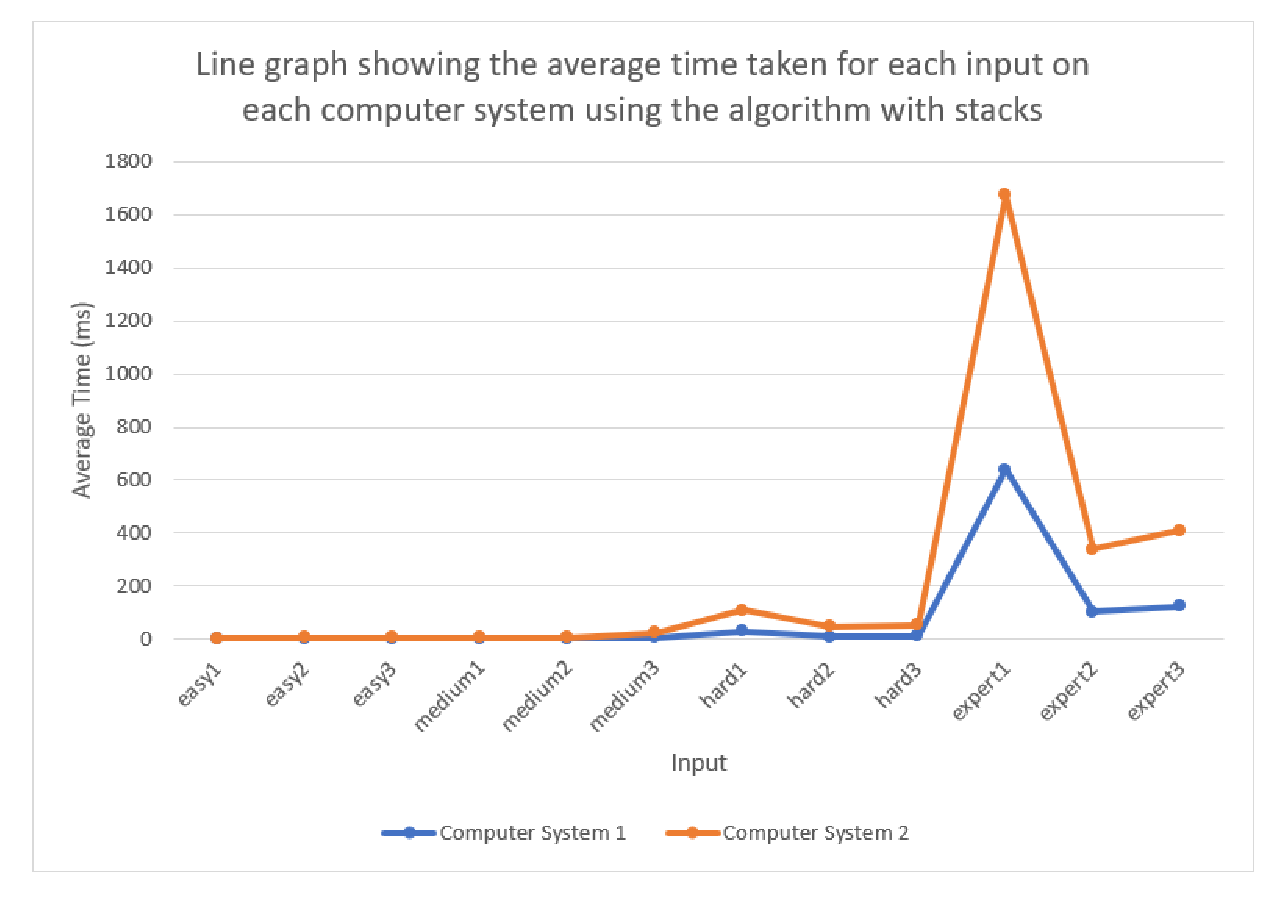
\includegraphics[scale=0.54]{fig5.eps}
\caption{ }
\end{figure}

\begin{figure}[H]
\centering
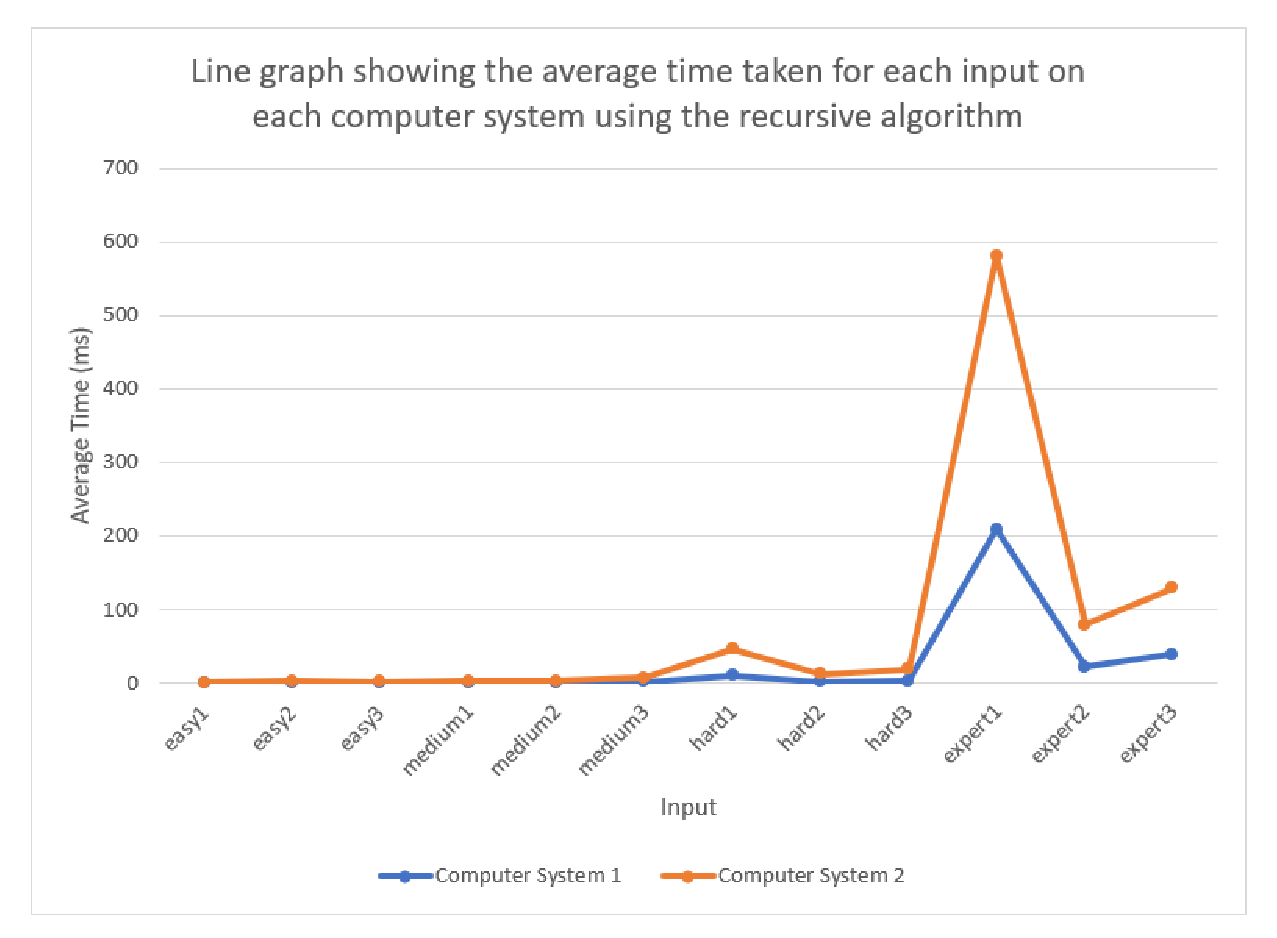
\includegraphics[scale=0.54]{fig6.eps}
\caption{ }
\end{figure}

\begin{figure}[H]
\centering
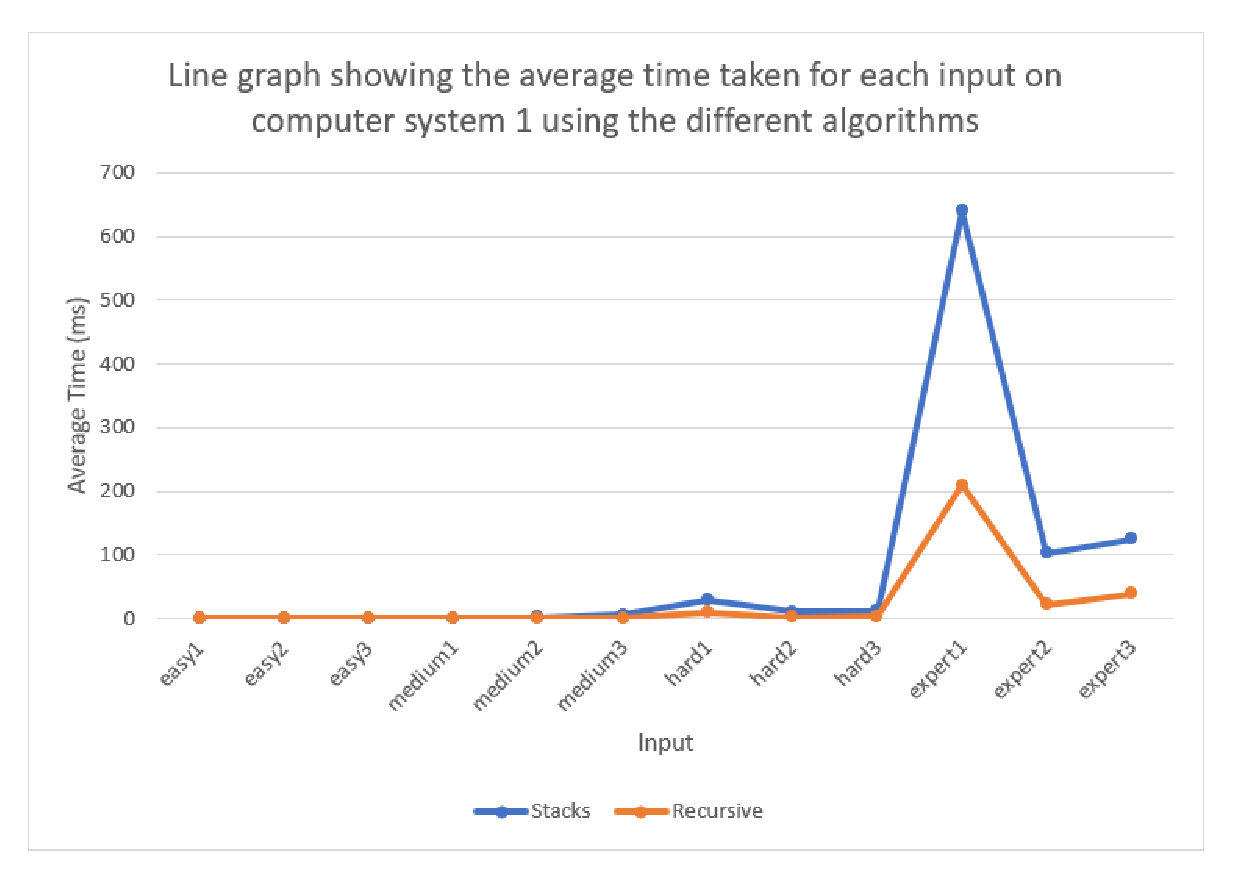
\includegraphics[scale=0.54]{fig7.eps}
\caption{ }
\end{figure}

\begin{figure}[H]
\centering
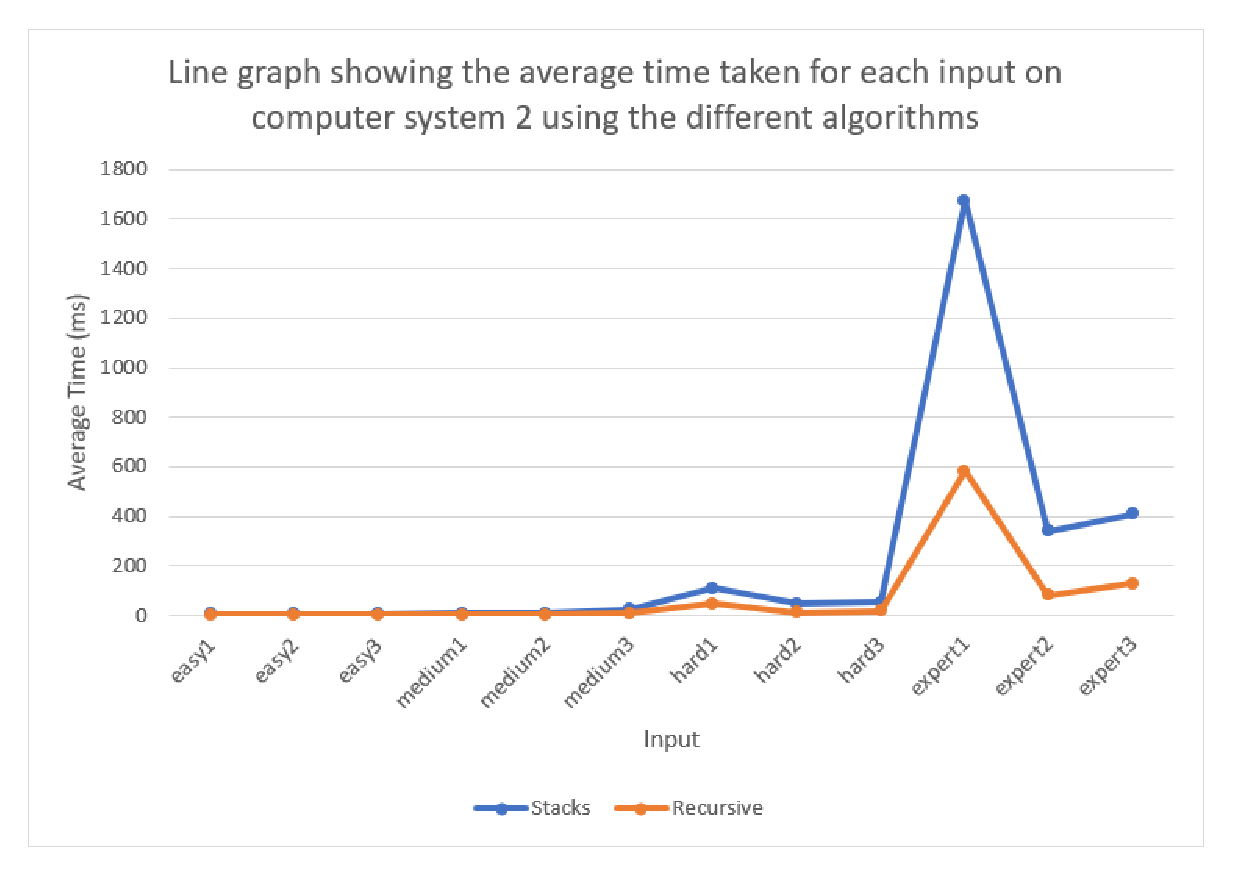
\includegraphics[scale=0.54]{fig8.eps}
\caption{ }
\end{figure}

\begin{figure}[H]
\centering
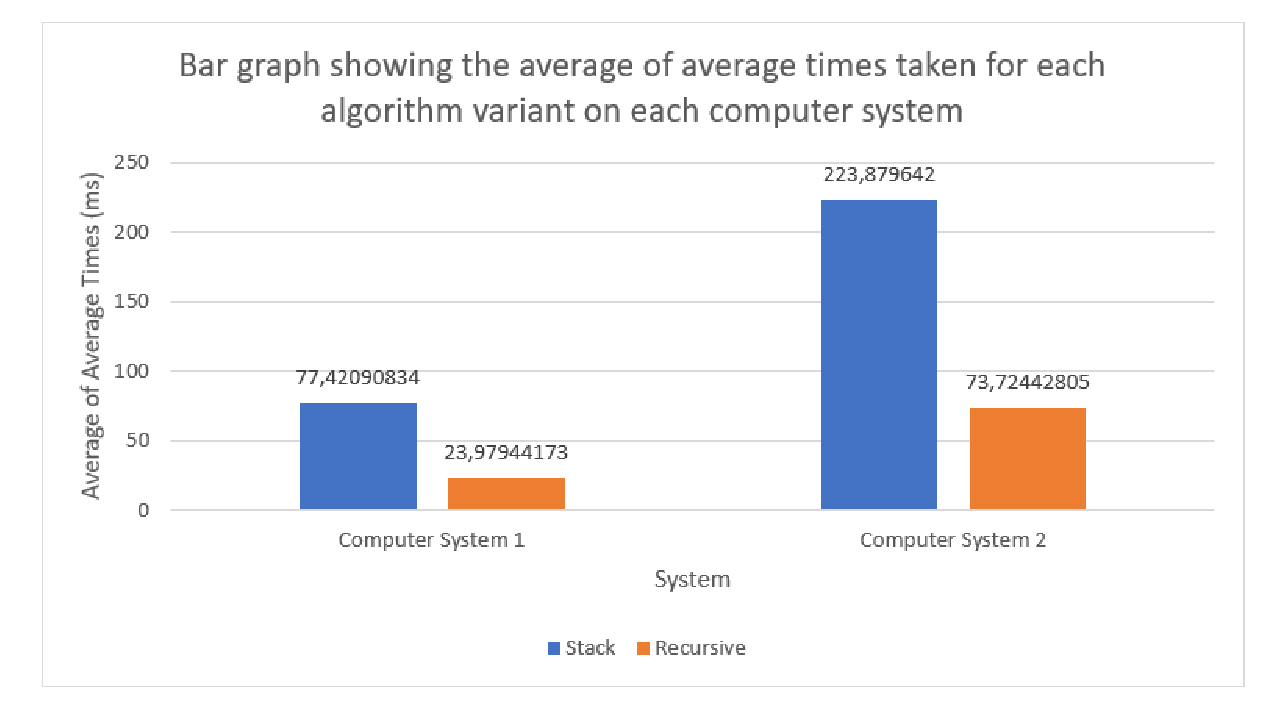
\includegraphics[scale=0.54]{fig9.eps}
\caption{ }
\end{figure}


\subsection{Number of empty elements affects runtime of each \\algorithm}
For this part of the experiment we will have a completed sudoku puzzle input into our algorithms. 
We will then have 5 element values removed at each iteration randomly and the resulting sudoku puzzle will be solved and the time will be recorded. 
For this part we will be testing both algorithm variants again but we will only run them on computer system 1. 
For this one we chose to use the expert2 sudoku puzzle. 
\\Here is an excerpt of how it ran:

\vspace{3mm} %5mm vertical space

Input
\\5 1 7 8 3 2 6 9 4 
\\9 3 6 7 4 5 8 1 2 
\\8 2 4 1 9 6 3 5 7 
\\4 5 9 6 1 3 7 2 8 
\\3 8 1 2 5 7 9 4 6 
\\7 6 2 9 8 4 1 3 5 
\\1 4 5 3 7 8 2 6 9 
\\2 9 8 5 6 1 4 7 3 
\\6 7 3 4 2 9 5 8 1

\vspace{3mm} %5mm vertical space

Iteration 1(remove 5 random elements)
\\5 1 7 8 0 2 6 9 4 
\\9 3 6 7 4 5 8 1 2 
\\8 2 4 1 9 6 3 5 0 
\\4 5 9 6 1 0 7 2 8 
\\3 8 1 2 5 7 9 4 6 
\\7 6 2 9 8 4 1 3 5 
\\1 4 5 3 7 8 2 6 9 
\\2 9 8 5 6 1 4 7 3 
\\6 7 3 4 0 0 5 8 1
\\Solve the sudoku puzzle above and record time

\vspace{3mm} %5mm vertical space

Iteration 2(remove another 5 random elements)
\\5 1 0 8 0 2 6 9 4 
\\9 3 6 7 4 5 8 1 2 
\\8 2 4 1 9 6 3 5 0 
\\0 5 9 6 1 0 7 2 8 
\\3 8 1 2 5 7 9 4 6 
\\7 6 2 0 8 4 0 3 5 
\\1 4 5 3 7 8 2 6 9 
\\0 9 8 5 6 1 4 7 3 
\\6 7 3 4 0 0 5 8 1
\\Solve the sudoku puzzle above and record time

\vspace{3mm} %5mm vertical space

This process was repeated until 21 populated elements remained.

\subsection{Tables of Results}

\begin{figure}[H]
\centering
\begin{tabular}{|l|l|}
\hline
Empty Cells & Time Taken(ms)\\
\hline
5	& 0,3081\\
10&	0,0567\\
15&	0,0931\\
20&	0,107\\
25&	0,1425\\
30&	0,2087\\
35&	0,1128\\
40&	0,4481\\
45&	1,0491\\
50&	2,5172\\
55&	2,7306\\
60&	1,5707\\
\hline
Average Time(ms) & 0,7787\\
\hline
\end{tabular}
\caption{the number of empty elements in a sudoku puzzle affects the time taken to be solved for the stacks implementation.}
\end{figure}

\begin{figure}[H]
\centering
\begin{tabular}{|l|l|}
\hline
Empty Cells & Time Taken(ms)\\
\hline
5	&0,0866\\
10&	0,0254\\
15&	0,0414\\
20&	0,0472\\
25&	0,0613\\
30&	0,0877\\
35&	0,0879\\
40&	0,1529\\
45&	0,102\\
50&	0,3318\\
55&	0,3548\\
60&	0,2557\\
\hline
Average Time(ms) & 0,1362\\
\hline
\end{tabular}
\caption{the number of empty elements in a sudoku puzzle affects the time taken to be solved for the recursive implementation.}
\end{figure}

\subsection{Graphs of Results}
\begin{figure}[H]
\centering
\includegraphics[scale=0.54]{fig12.eps}
\caption{ }
\end{figure}

\section{Interpretation of Results}
From the results above, we can clearly see that the single core performance of the computer system on which the algorithm is run has a significant impact on the run time. 
For both algorithms used, the run time to solve the 
puzzles on computer system 1 is 3-4 times less than that on computer system 2. 

\vspace{3mm}

From the line graphs above, it can be observed that each algorithm seems to trend the same on each computer system due to the fact that both graphs have the same shape. 
We can also see that our backtracking algorithm involving stacks is considerably more inefficient than the recursive implementation of the backtracking algorithm. 
This is further supported by the bar graph above which shows that the stacks algorithm runs 3-4 times slower than the recursive implementation in identical conditions on the same puzzle.\\ 

\vspace{3mm}

The reason for this is due to the fact that the chosen method of stack implementation is inefficient. 
The recursive solving of the sudoku puzzle involves trying different number combinations where there are zeroes by calling the same solve function. 
If the algorithm finds correct values for 3 elements and then realizes that it cannot be solved further, 
it can backtrack quickly, even if it has to go back to the first element by returning false and setting all updated element values back to 0.

\vspace{3mm}

The stack implementation of the backtracking algorithm finds the first zero and pushes the first value to try which would be 1 to the stack. 
It also pushes the x and y coordinate of the value to two other stacks respectively. If the value of one 1 did not work in that position then the algorithm will pop from the values stack, 
as well as the two coordinate stacks and then try the next value 2 in that x and y coordinate. It will also push the same x and y co-ordinate values to the stacks again. 
These stack operations of pushing and popping make a significant contribution to the lengthy run time of this implementation. If all 3 elements are correctly placed and then the algorithm 
reaches a point where the puzzle cannot be solved further, it backtracks slowly if it has to go back to the first element due to the numerous peeks and pops needed. 
Each x and y coordinate pair will need to peeked and popped and the value set back to 0. In this example there will be 3 peeks and pops each for the x and y coordinates. 
The algorithm will also need to perform three pops and a peek in total on the value stack. This is a total of 16 peek/pop operations to backtrack to the first element, 
compared to a maximum of 3 operations in the recursive implementation. Due to these operations, 
this stack implementation can become considerably slower than the recursive one depending on the size of the puzzle and number of missing elements.

\vspace{3mm}

For the results regarding the relation between the number of populated elements in a sudoku puzzle and the time taken to solve it, 
a general increase in run time as the number of populated elements decreases can be observed. The times taken using the stack algorithm with regards to this test are also higher 
than the times recorded by the recursive implementation which also further supports the assertion that our stack implementation is worse than the recursive implementation.

\section{Relate results to Theory}
As seen in figures 1 through to figure 4, although the runtime of the algorithm increases as the complexity of the puzzle increases, 
the extent of this increase is not proportionate to the number of empty cells but rather to the number of attempts needed to generate a correct solution. 
This is prevalent in the runtime of the three expert level puzzles used to generate the result data with puzzle “expert 2” 
having a significantly higher runtime than puzzles “expert 1” and “expert 3”. The graphics in figures 5 to 8 show that there is no polynomial 
representation for the solving of a sudoku puzzle using either implementation of the backtracking algorithm and supports the theoretical statement that this problem has a 
nondeterministic polynomial.

\vspace{3mm}

Figure 12 shows a graph of the time complexity of solving a sudoku puzzle with N empty cells. T
he theoretical time complexity of solving a 9-by-9 puzzle is known to be exponential. This is supported by the overall shape of the two graphs and is more pronounced in 
the stack implementation due to the longer and more inefficient runtime. Thus, our empirical analysis agrees with the theoretical analysis. It also helps us come to the 
conclusion that the more populated elements you have in a sudoku puzzle, the more likely it will be solved quicker when using the backtracking algorithm.

\section{Conclusion}
In this experiment we set out to explore the performance of the backtracking algorithm in solving a 9-by-9 sudoku puzzle. The time-based performance of both a recursive and 
a stack implementation of the algorithm were measured and compared with each other. In order to further understand the performance of the algorithm the algorithms were run on 
different computer hardware in order to obtain additional data and rule out any inaccuracies due to bottlenecking. 
Additional tests on the runtime of the algorithm were also run on puzzles with different numbers of unpopulated cells in order to measure the performance and runtime. 

\vspace{3mm}

The experiments were run on puzzles of different levels of difficulty multiple times and the results averaged in order to obtain accurate results. 
These results supported the theoretical analysis that the backtracking 
algorithm when solving a sudoku puzzle has a non-deterministic polynomial and that the time taken is dependent on the number of attempts made by the algorithm. 

\vspace{3mm}

In the second part of this experiment it was found that the empirical data supports the assertion that the theoretical time complexity of solving a 9-by-9 puzzle is exponential. 

\vspace{3mm}

In using both a stack and recursive implementation we were able to compare the effect implementation has on the overall performance on the runtime of the algorithm. 
It was observed that using recursion is considerably more efficient and thus implementation and optimisation is essential to the performance of the backtracking algorithm. 

\vspace{3mm}

Whilst every attempt was made to avoid errors in measurement by running the experiments without background tasks it is possible that our results may have been affected by other 
processes and may have resulted in slightly skewed and less accurate results. 

\vspace{3mm}

The experiments conducted could be extended to include additional sudoku puzzles of size N-by-N which would allow for further investigation of the NP-complete nature of an N-by-N 
sudoku puzzle as well as allow for the observation of the effect the dimensions of the puzzle have on the exponential performance of the algorithm when comparing the runtimes with empty cells. 
Further implementation methods could also be considered in order to determine the most efficient method of implementing the backtracking algorithm in order to maximize performance. 

\newpage
% References
\bibliographystyle{unsrt}
\bibliography{Project}

\newpage
% Appendices
\begin{appendices}
\section{Backtracking Implementation Using Stacks}
%code
\begin{lstlisting}
import java.util.Scanner;
import java.util.Stack;

public class Program {
    void PrintGrid(char[][] grid) {
        for (int i = 0; i < 9; i++) {
            for (int j = 0; j < 9; j++) {
                System.out.print(grid[i][j] + " ");
            }
            System.out.println();
        }
    }

    boolean IsInValidState(char[][] grid, int row, int col) {
        if (grid[row][col] == '0') {
            return false;
        }
        for (int m = 0; m < 9; ++m) {
            if (grid[row][m] == grid[row][col] && m != col) {
                return false;
            } else if (grid[m][col] == grid[row][col] && m != row) {
                return false;
            }
        }
        int X_0 = (row / 3) * 3;
        int Y_0 = (col / 3) * 3;
        for (int i = 0; i < 3; ++i) {
            for (int j = 0; j < 3; ++j) {
                if (grid[X_0 + i][Y_0 + j] == grid[row][col] 
                    && !(X_0 + i == row && Y_0 + j == col)) {
                    return false;
                }
            }
        }
        return true;
    }


    void solveSudoku(char[][] grid) {
        Timer myTimer = new Timer();
        myTimer.start();
        Stack<Integer> sRow = new Stack<>();
        Stack<Integer> sCol = new Stack<>();
        Stack<Character> sValue = new Stack<>();
        int row = 0;
        int col = 0;
        int shape = 9;
        char cShape = (char) ('0' + (char) shape);
        boolean Print = true;
        boolean bFinished = false;
        for (int r = 0; r < 9; r++) {
            for (int c = 0; c < 9; c++) {
                if (grid[r][c] == '0') {
                    bFinished = true;
                    row = r;
                    col = c;
                    break;
                }
            }
            if (bFinished) {
                break;
            }
        }

        while (bFinished) {
            while (!IsInValidState(grid, row, col) 
                    && grid[row][col] != cShape) {
                char tmp = grid[row][col];
                int itmp = tmp - 48;
                itmp = itmp + 1;
                tmp = (char) ('0' + (char) itmp);
                grid[row][col] = tmp;
            }
            if (IsInValidState(grid, row, col)) {
                sRow.push(row);
                sCol.push(col);
                sValue.push(grid[row][col]);
                bFinished = false;
                for (int r = 0; r < 9; r++) {
                    for (int c = 0; c < 9; c++) {
                        if (grid[r][c] == '0') {
                            bFinished = true;
                            row = r;
                            col = c;
                            break;
                        }
                    }
                    if (bFinished) {
                        break;
                    }
                }
            } else if (sValue.empty()) {
                System.out.println("No Solution");
                Print = false;
                bFinished = false;
            } else {
                grid[row][col] = '0';
                row = sRow.peek();
                col = sCol.peek();
                sValue.peek();
                sRow.pop();
                sCol.pop();
                sValue.pop();
                while (grid[row][col] == cShape) {
                    grid[row][col] = '0';
                    row = sRow.peek();
                    col = sCol.peek();
                    sValue.peek();
                    sRow.pop();
                    sCol.pop();
                    sValue.pop();
                }
                char tmp = grid[row][col];
                int itmp = tmp - 48;
                itmp = itmp + 1;
                tmp = (char) ('0' + (char) itmp);
                grid[row][col] = tmp;
            }
        }
        myTimer.stop();
        if (Print) {
            PrintGrid(grid);
            System.out.println("Time: " + myTimer.getTime());
        }
    }

    public static void main(String[] args) {
        Scanner scanner = new Scanner(System.in);
        //read in data

        char[][] grid = new char[9][9];
        for (int k = 0; k < 9; k++) {
            String line = scanner.nextLine();
            String[] nums = line.split(" ");
            for (int i = 0; i < 9; i++) {
                grid[k][i] = nums[i].charAt(0);
            }
        }

        Program ob = new Program();
        ob.solveSudoku(grid);
    }
}
\end{lstlisting}

\newpage
\section{Backtracking Implementation Using Recursion}
This algorithm was retrieved from website \cite{art6}, and is solely used for 
comparison purposes against our algorithm which utilises stacks.

\vspace{3mm}
% Code
\begin{lstlisting}
import java.util.Scanner;

public class Program {

    public static void main(String[] args) {
        /*Inputting grid */
        int[][] grid = new int[9][9];
        Scanner in = new Scanner(System.in);
        for (int k = 0; k < 9; k++) {
            String line = in.nextLine();
            String[] nums = line.split(" ");
            for (int i = 0; i < 9; i++) {
                grid[k][i] = Integer.parseInt(nums[i]);
            }
        }

        /*Solving grid */
        Timer myTimer = new Timer();
        myTimer.start();
        boolean solve = solve(grid, grid.length);
        myTimer.stop();

        if (solve) {
            print(grid);
        } else {
            System.out.println("No solution");
        }
        System.out.println("Time: " + myTimer.getTime());
    }

    public static boolean solve(int[][] grid, int n) {
        // int solved[][] = grid;
        int row = -1, col = -1;
        boolean flag = true;
        for (int i = 0; i < n; i++) {
            for (int j = 0; j < n; j++) {
                if (grid[i][j] == 0) {
                    row = i;
                    col = j;
                    flag = false;
                    break;
                }
            }
            if (!flag) {
                break;
            }
        }

        if (flag) {
            return true;
        } else {
            for (int value = 1; value <= n; value++) {
                if (validState(grid, row, col, value)) {
                    grid[row][col] = value;
                    if (solve(grid, n)) {
                        return true;
                    } else {
                        grid[row][col] = 0;
                    }

                }
            }
        }
        return false;
    }

    public static boolean validState
    (int[][] grid, int row, int col, int n) {
        int len = grid.length;
        for (int i = 0; i < len; i++) {
            if (grid[row][i] == n || grid[i][col] == n) {
                return false;
            }
        }

        int sqrtLen = (int) Math.sqrt(len);
        int StartRow3x3 = row - row % sqrtLen;
        int StartCol3x3 = col - col % sqrtLen;

        for (int k = StartRow3x3; 
              k < StartRow3x3 + sqrtLen; k++) {
            for (int l = StartCol3x3; l < StartCol3x3 + sqrtLen; l++) {
                if (grid[k][l] == n) {
                    return false;
                }
            }
        }

        return true;
    }


    public static void print(int[][] grid) {
        for (int i = 0; i < 9; i++) {
            for (int j = 0; j < 9; j++) {
                System.out.print(grid[i][j] + " ");
            }
            System.out.println();
        }
    }
}

\end{lstlisting}

\newpage
\section{Timer Class}
% Code
\begin{lstlisting}
import static java.lang.System.nanoTime;

public class Timer{
    public long startTime;
    public long endTime;

    public void start(){
        startTime = nanoTime();
    }

    public void stop(){
        endTime = nanoTime();
    }

    public double getTime(){
        return (double) (endTime - startTime) / 1000000;
    }
}
\end{lstlisting}

\newpage
\section{Backtracking Stack Implementation for Cell Count Experiment}
% Code
\begin{lstlisting}
import java.util.Scanner;
import java.util.Random;
import java.util.Sk;

public class Program {
    public static void PrintGrid(char[][] grid) {
        for (int i = 0; i < 9; i++) {
            for (int j = 0; j < 9; j++) {
                System.out.print(grid[i][j] + " ");
            }
            System.out.println();
        }
    }

    boolean IsInValidState(char[][] grid, 
                            int row, int col) {
        if (grid[row][col] == '0') {
            return false;
        }
        for (int m = 0; m < 9; ++m) {
            if (grid[row][m] == grid[row][col] &
                & m != col) {
                return false;
            } else if (grid[m][col] == grid[row][col] 
                && m != row) {
                return false;
            }
        }
        int X_0 = (row / 3) * 3;
        int Y_0 = (col / 3) * 3;
        for (int i = 0; i < 3; ++i) {
            for (int j = 0; j < 3; ++j) {
                if (grid[X_0 + i][Y_0 + j] == grid[row][col] 
                && !(X_0 + i == row && Y_0 + j == col)) {
                    return false;
                }
            }
        }
        return true;
    }


    void solveSudoku(char[][] grid) {
        Timer myTimer = new Timer();
        myTimer.start();
        Stack<Integer> sRow = new Stack<>();
        Stack<Integer> sCol = new Stack<>();
        Stack<Character> sValue = new Stack<>();
        int row = 0;
        int col = 0;
        int shape = 9;
        char cShape = (char) ('0' + (char) shape);
        boolean Print = true;
        boolean bFinished = false;
        for (int r = 0; r < 9; r++) {
            for (int c = 0; c < 9; c++) {
                if (grid[r][c] == '0') {
                    bFinished = true;
                    row = r;
                    col = c;
                    break;
                }
            }
            if (bFinished) {
                break;
            }
        }

        while (bFinished) {
            while (!IsInValidState(grid, row, col) 
            && grid[row][col] != cShape) {
                char tmp = grid[row][col];
                int itmp = tmp - 48;
                itmp = itmp + 1;
                tmp = (char) ('0' + (char) itmp);
                grid[row][col] = tmp;
            }
            if (IsInValidState(grid, row, col)) {
                sRow.push(row);
                sCol.push(col);
                sValue.push(grid[row][col]);
                bFinished = false;
                for (int r = 0; r < 9; r++) {
                    for (int c = 0; c < 9; c++) {
                        if (grid[r][c] == '0') {
                            bFinished = true;
                            row = r;
                            col = c;
                            break;
                        }
                    }
                    if (bFinished) {
                        break;
                    }
                }
            } else if (sValue.empty()) {
                System.out.println("No Solution");
                Print = false;
                bFinished = false;
            } else {
                grid[row][col] = '0';
                row = sRow.peek();
                col = sCol.peek();
                sValue.peek();
                sRow.pop();
                sCol.pop();
                sValue.pop();
                while (grid[row][col] == cShape) {
                    grid[row][col] = '0';
                    row = sRow.peek();
                    col = sCol.peek();
                    sValue.peek();
                    sRow.pop();
                    sCol.pop();
                    sValue.pop();
                }
                char tmp = grid[row][col];
                int itmp = tmp - 48;
                itmp = itmp + 1;
                tmp = (char) ('0' + (char) itmp);
                grid[row][col] = tmp;
            }
        }
        myTimer.stop();
        if (Print) {
            PrintGrid(grid);
            System.out.println("Time: " + 
            String.valueOf(myTimer.getTime()));
        }
    }

    public static void main(String[] args) {
        Scanner scanner = new Scanner(System.in);
        //read in data

        char[][] grid = new char[9][9];
        char[][] changedGrid = new char[9][9];
        for (int k = 0; k < 9; k++) {
            String line = scanner.nextLine();
            String[] nums = line.split(" ");
            for (int i = 0; i < 9; i++) {
                grid[k][i] = nums[i].charAt(0);
                changedGrid[k][i] = nums[i].charAt(0);
            }
        }

        int totCount = 80;
        Random rand = new Random(1);
        while (totCount >= 22) {
            System.out.println("Input grid");
            int count = 5;
            totCount = totCount - count;
            System.out.println("totCount populated: " + totCount);
            while (count > 0) {
                int rowChange = rand.nextInt(9);
                int colChange = rand.nextInt(9);
                if (changedGrid[rowChange][colChange] != '0') {
                    grid[rowChange][colChange] = '0';
                    changedGrid[rowChange][colChange] = '0';
                    count = count - 1;
                }
            }
            PrintGrid(grid);
            Program ob = new Program();
            System.out.println("Output grid");
            ob.solveSudoku(grid);
            for (int k = 0; k < 9; k++) {
                System.arraycopy(changedGrid[k], 0, grid[k], 0, 9);
            }
        }

    }
}

\end{lstlisting}

\newpage
\section{Backtracking Recursive Implementation for Cell Count Experiment}
This algorithm was adapted from the code found from website \cite{art6}, 
and is solely used for comparison purposes against our 
algorithm which utilises stacks again.

\vspace{3mm}
% Code
\begin{lstlisting}
import java.util.Scanner;
import java.util.Random;

public class Program {

    public static void main(String[] args) {
        /*Inputting grid */
        int[][] grid = new int[9][9];
        int[][] changedGrid = new int[9][9];
        Scanner in = new Scanner(System.in);
        for (int k = 0; k < 9; k++) {
            String line = in.nextLine();
            String[] nums = line.split(" ");
            for (int i = 0; i < 9; i++) {
                grid[k][i] = Integer.parseInt(nums[i]);
                changedGrid[k][i] = Integer.parseInt(nums[i]);
            }
        }

        int totCount = 80;
        Random rand = new Random(1);
        while (totCount >= 22) {
            System.out.println("Input grid");
            int count = 5;
            totCount = totCount - count;
            System.out.println("totCount populated: " + totCount);
            while (count > 0) {
                int rowChange = rand.nextInt(9);
                int colChange = rand.nextInt(9);
                if (changedGrid[rowChange][colChange] != 0) {
                    grid[rowChange][colChange] = 0;
                    changedGrid[rowChange][colChange] = 0;
                    count = count - 1;
                }
            }
            print(grid);
            Program ob = new Program();
            System.out.println("Output grid");
            /*Solving grid */
            Timer myTimer = new Timer();
            myTimer.start();
            boolean solve = solve(grid, grid.length);
            myTimer.stop();
            if (solve) {
                print(grid);
            } else {
                System.out.println("No solution");
            }
            System.out.println("Time: " + 
                        String.valueOf(myTimer.getTime()));
            for (int k = 0; k < 9; k++) {
                System.arraycopy(changedGrid[k], 0, grid[k], 0, 9);
            }
        }
    }

    public static boolean solve(int[][] grid, int n) {
        // int solved[][] = grid;
        int row = -1, col = -1;
        boolean flag = true;
        for (int i = 0; i < n; i++) {
            for (int j = 0; j < n; j++) {
                if (grid[i][j] == 0) {
                    row = i;
                    col = j;
                    flag = false;
                    break;
                }
            }
            if (!flag) {
                break;
            }
        }

        if (flag) {
            return true;
        } else {
            for (int value = 1; value <= n; value++) {
                if (validState(grid, row, col, value)) {
                    grid[row][col] = value;
                    if (solve(grid, n)) {
                        return true;
                    } else {
                        grid[row][col] = 0;
                    }

                }
            }
        }
        return false;
    }

    public static boolean validState(int[][] grid, 
                                    int row, int col, int n) {
        int len = grid.length;
        for (int i = 0; i < len; i++) {
            if (grid[row][i] == n || grid[i][col] == n) {
                return false;
            }
        }

        int sqrtLen = (int) Math.sqrt(len);
        int StartRow3x3 = row - row % sqrtLen;
        int StartCol3x3 = col - col % sqrtLen;

        for (int k = StartRow3x3; k < StartRow3x3 + sqrtLen; k++) {
            for (int l = StartCol3x3; 
                        l < StartCol3x3 + sqrtLen; l++) {
                if (grid[k][l] == n) {
                    return false;
                }
            }
        }

        return true;
    }


    public static void print(int[][] grid) {
        for (int i = 0; i < 9; i++) {
            for (int j = 0; j < 9; j++) {
                System.out.print(grid[i][j] + " ");
            }
            System.out.println("");
        }
    }
}

\end{lstlisting}


\end{appendices}

\end{document}
